\chapter{Results}
\label{ch:results}

In this chapter, we evaluate the results of the simulations that were designed in the previous chapter \ref{ch:experiments}.

There are too many different situations, to evaluate each setup completely. Moreover, each situation can be modeled in the developed simulation framework that is part of the published source code~\cite{fidesGithub} and thus anybody can verify and simulate their own situation they are interested in.

For that reason, we focus mainly on evaluating Fides under specific conditions that verify its resilience in the situations with many byzantine peers.
We try to discover a situation where there are as much adversarial peers as possible and Fides is still able to guarantee that it is able to come up with correct target score.

Note, that all all figures in this chapter can be replicated by re-running the simulations that are stored in the package with the implementation $simulations/cases/figures$~\cite{fidesGithub}.
The graphs might be slightly different because the threat intelligence and recommendations are sampled as described in \ref{sec:sampling-threat-intelligence}, but the overall results should be the same.

\section{General Overview of a Single Simulation}
\label{sec:general-overview-of-simulation-output}
To understand the results of our simulation we first need describe how does the outcome of a simulation looks like, such as the example shown in Figure~\ref{fig:single-simulation-example}.
The simulation framework provides this graph for each possible simulation.

\begin{figure}
    \centering
    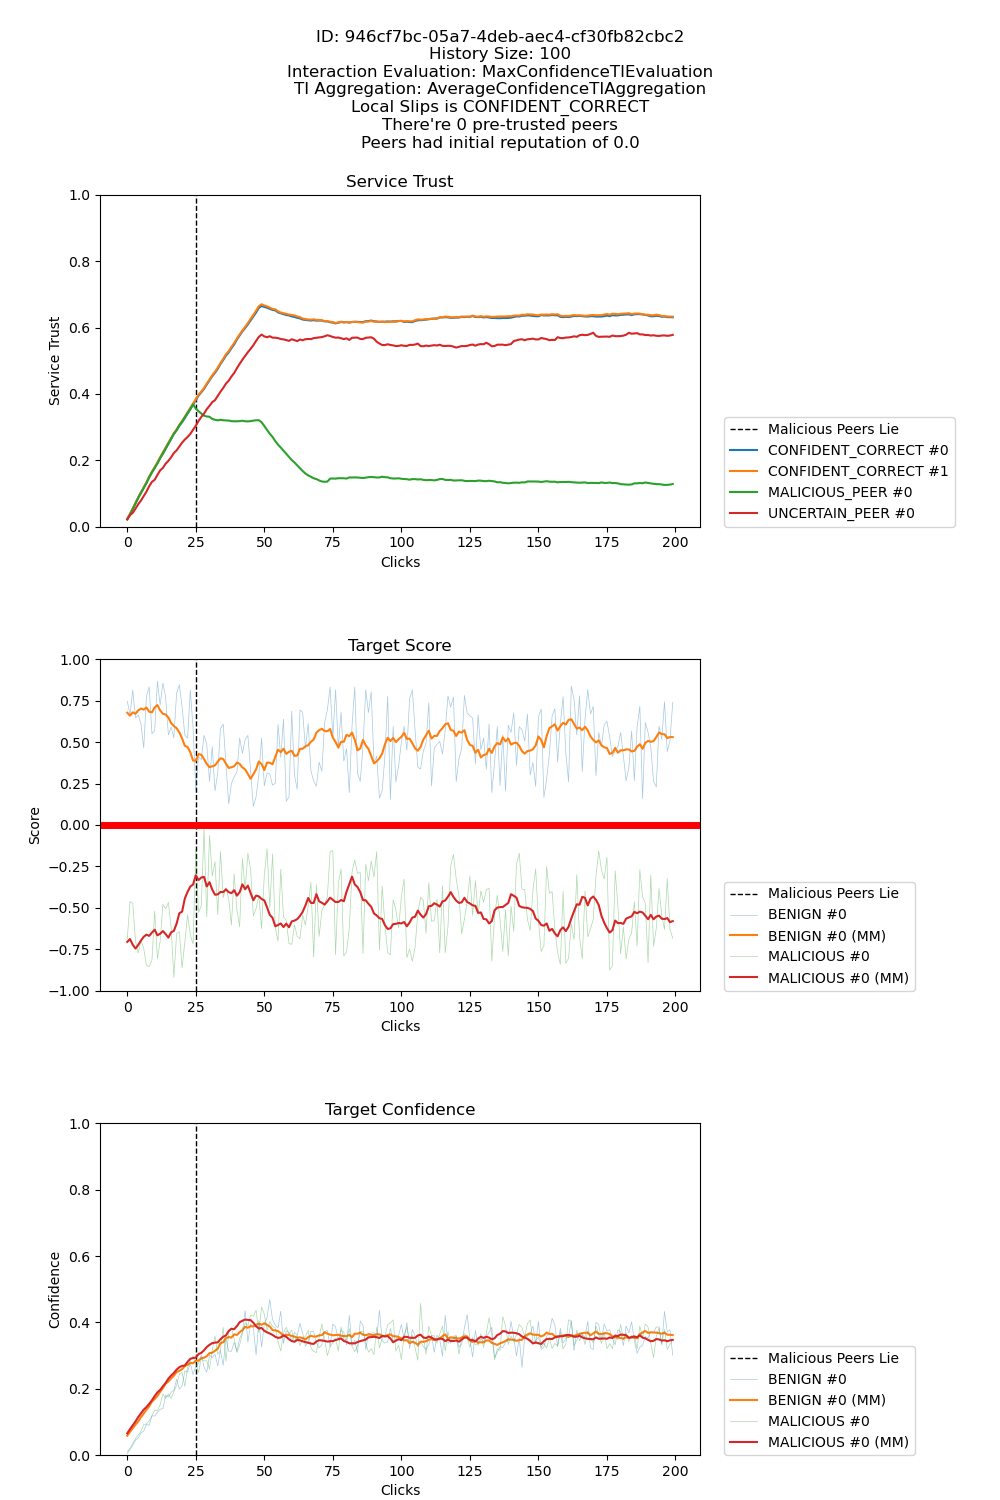
\includegraphics[width=0.83\textwidth]{assets/example_evaluation.png}
    \caption{An example outcome from a single simulation. The graph on top shows how \textit{service trust} changes as time goes by. In this example there are four peers, two confident correct, one uncertain and one malicious. The graph in the middle shows the score for the targets as computed by Fides based on what the peers said. There are two targets (imagine \textit{google.com} and \textit{evil.com}) and Fides computes the score for each of them: 1 means benign, -1 means malicious. The lower graph shows the aggregated confidence for the same targets. That means how confident is Fides about the score in the middle graph.}
    \label{fig:single-simulation-example}
\end{figure}

The graph's headline explains which setup parameters were used for the trust model. In the case of Figure~\ref{fig:single-simulation-example} Fides used the interaction evaluation strategy $MaxConfidenceTIEvaluation$ (Section~\ref{subsec:MaxConfidenceTIEvaluation}).
For aggregating threat intelligence, Fides used the aggregation described in Section~\ref{sec:network-intelligence-aggregation}.
The local Slips instance behaved like a confident correct peer outlined in Section~\ref{subsubsec:confident-correct-peer}.

The graph on top in Figure~\ref{fig:single-simulation-example} shows the development of the \textit{service trust} $st_{i, j}$ (Section~\ref{subsec:service-trust}) on the vertical axis over \textit{time} on the horizontal axis. As mentioned in Section~\ref{sec:environment-simulation}, the time is measured in \textit{clicks}.
The higher the service trust is for a peer, the higher impact it has on the final aggregated threat intelligence.
One can see multiple peers that were involved in the simulation and their respective behavior. All possible behaviors are described in Section~\ref{sec:peers-behavioral-patterns}.
There were four different peers that were communicating with the local instance of Fides, two of them were \textit{confident correct}, one was an \textit{uncertain peer} and the last one was a \textit{malicious peer}.

The dotted line indicates the time when the malicious peers start lying.
One can see that during this first period, when the malicious peers were not lying \textit{(before the line)}, they were gaining the service trust.
In the case of Figure~\ref{fig:single-simulation-example} this happened at click 25 when the malicious peers started lying.
After that, it is clear that they started to lose the service trust.

The second graph in Figure~\ref{fig:single-simulation-example} shows the \textit{target score} during the time (\textit{clicks}).
The target score $S^{k}_{T}$ (Section~\ref{sec:network-intelligence-aggregation}) is the part of the aggregated network threat intelligence, that was computed from the scores and confidences provided by each peer.
The score was calculated by Fides at click $k$ for target $T$.

The score graph contains two different targets, one that is according to the ground truth malicious and a second one that was benign.
We also included the moving average value (indicated as MM) within the window of 10 clicks to make the graph clear.

Finally, the third graph, displays the aggregated confidence $C^{k}_{T}$ (Section~\ref{sec:network-intelligence-aggregation}) over time (\textit{clicks}).
The graph is similar to the score, we include raw values for each time window and target, as well as the moving average within the window of 10 clicks.

In this example output graph, it can be seen that Fides was clearly able to identify that the malicious peer started to lie after click 25 because of the service trust $st^{k}_{i,j}$ for this peer that fell down almost instantly.
At the same time, we can see that on the score graph, the $S^{k}_{T}$ for both targets were skewed and started to get closer to $0$ because the malicious peer had already gained service trust and thus the threat intelligence provided by it had an impact on the final $S^{k}_{T}$.
However, after Fides identified that the peer is lying, it lowered the service trust for this peer, and the score started to recover closer to the baseline.

\section{Evaluation of Fides Resilience in Different Scenarios}
\label{sec:fides-resilience}

To evaluate the resilience of Fides in different scenarios, we need to find the optimal configuration for the following parameters in Fides: interaction evaluation strategy (Section~\ref{sec:interaction-evaluation-strategies}), threat intelligence aggregation function (Section~\ref{sec:network-intelligence-aggregation}) and initial reputation (Section~\ref{subsubsec:computing-reputation}). Each combination of parameters is evaluated in its capacity to correctly classify targets in \textit{any} network topology.\footnote{Distribution of correct/uncertain/incorrect/malicious peers in the network.}
In other words, what setup should the Fides's administrator use in order for Fides to guarantee that it will be able to \textit{eventually} classify targets correctly.

We discovered that actually there \textbf{exists} a particular setup that guarantees that Fides is able to eventually classify the targets correctly in a very adversarial situation. When Fides communicates with at least 25\% of pre-trusted peers from pre-trusted organizations ($0.25 \cdot |P|$ are pre-trusted) and uses $DistanceBasedTIEvaluation$ (section~\ref{subsec:distance-based-eval}) for evaluating the interactions in combination with $AverageConfidenceTIAggregation$ (Section~\ref{subsec:AverageConfidenceTIAggregation}) for aggregating the threat intelligence; then Fides is able to correctly classify the targets no matter how many adversarial peers are in the network (up to filling the remaining 75\%) or how hard they lie.

\subsection{Correct Target Identification Under Harsh Conditions}
\label{subsec:correct-target-identification-no-matter-what}

The first scenario that was evaluated was when the network has 25\% of pre-trusted peers. Several configurations were simulated, which results are shown in Figure~\ref{fig:performance-all-setups-25-pretrusted}.
There are three rows and four columns. Each row contains a single interaction evaluation strategy (Section~\ref{sec:interaction-evaluation-strategies}) and each column contains a single metric that evaluates the behavior of that strategy in the network.
There are three different metrics that evaluate the performance of the Fides's setup and the last graph displays how many confident correct (Section~\ref{subsubsec:confident-correct-peer}) peers there are in the network.
The horizontal axis in each graph measures the environment hardness explained in Section~\ref{subsec:environment-hardness}.
The vertical axis is different for each metric.

As mentioned previously, there are three different metrics.
The first column is a metric measuring target detection performance~(\ref{subsec:target-detection-performance-metric}), the second is the peers' behavior detection metric~(\ref{subsec:peers-behavior-detection-performance-metric}) and the third column then measures the average service trust $st^{kmax}_{i, j}$ for all peers in the simulation.

The last, fourth, column then contains a graph that displays what percentage of peers in the simulation were confident correct~(\ref{subsubsec:confident-correct-peer}) with respect to the environment hardness value~(\ref{subsec:environment-hardness}).
We include it in the graph to allow better visualization of how does the simulation environment looks like with respect to the peer's distribution.

\begin{figure}[hp!]
    \centering
    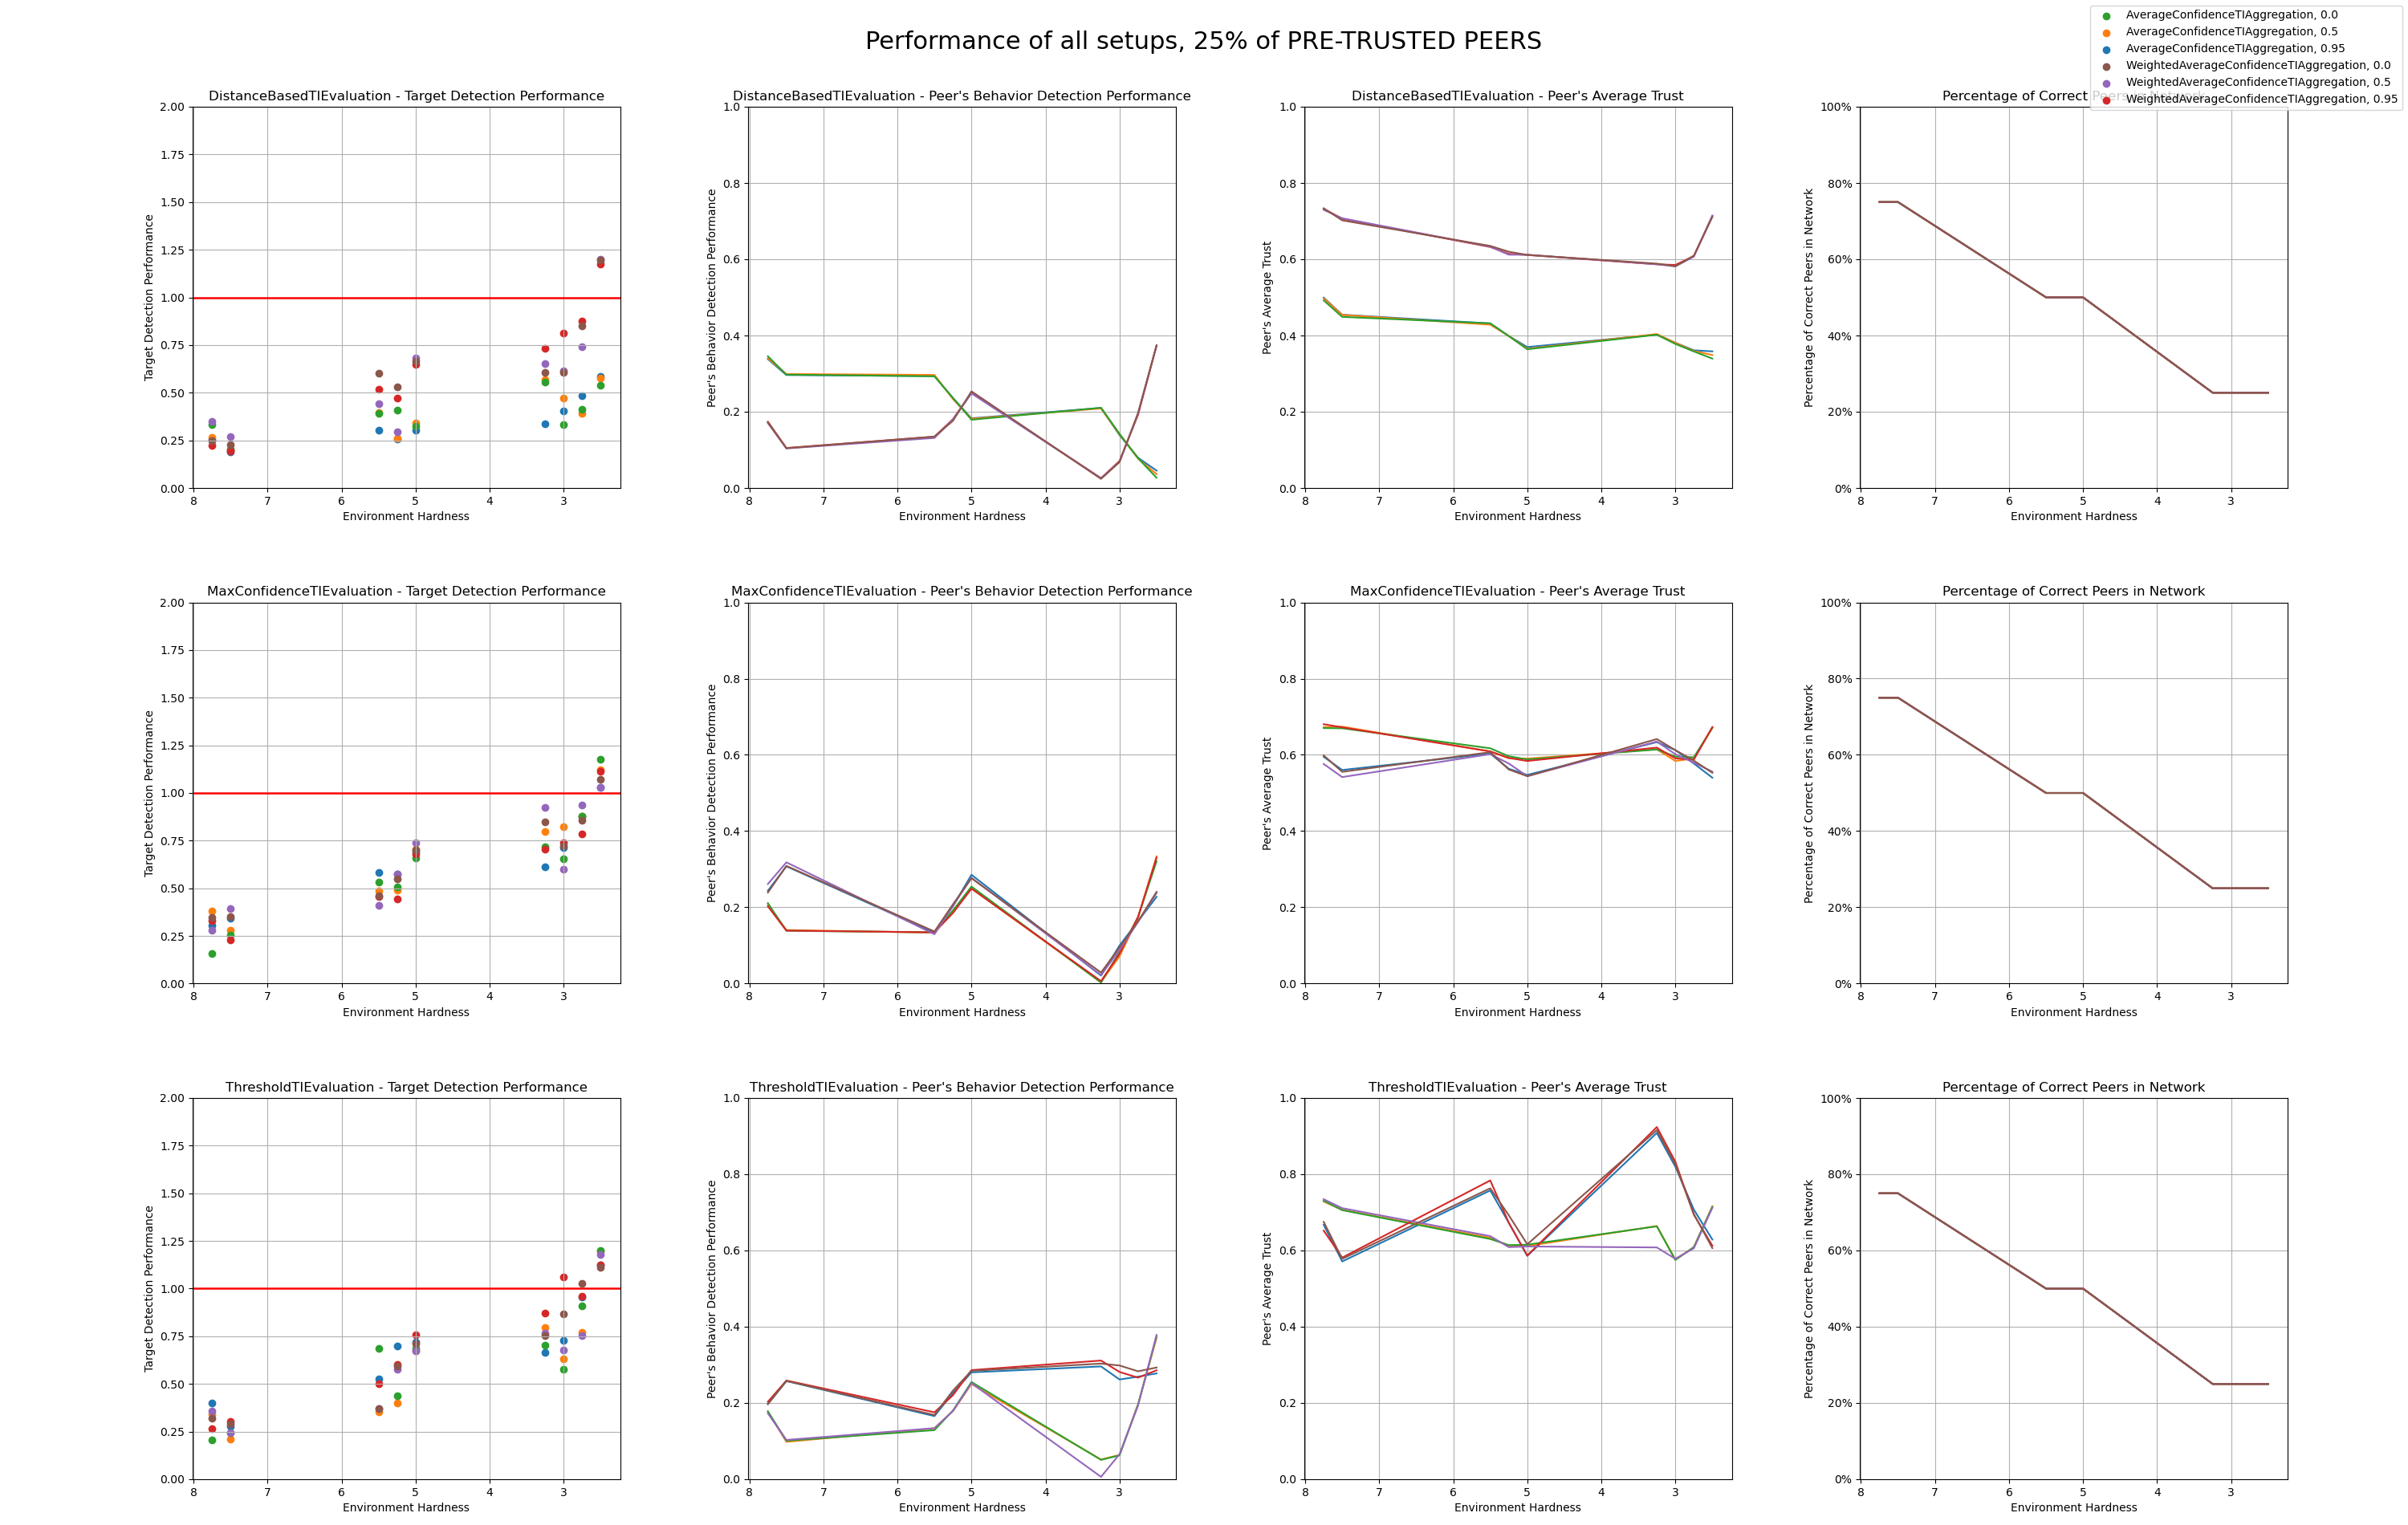
\includegraphics[width=0.94\paperwidth, angle=90]{assets/25_all_metrics.png}
    \caption{Performance of all setups with 25\% pre-trusted peers}
    \label{fig:performance-all-setups-25-pretrusted}
\end{figure}

The most important metric is the target detection performance~(\ref{subsec:target-detection-performance-metric}), which is visualized on the first graph.
A single dot in the graph is the value of $tdp$ and in a case when the $tdp \geq 1$, it means that Fides made on average the wrong decision about the targets and classified them with the wrong label.
In other words, if $tdp \geq 1$, Fides classified benign targets as malicious and the other way around.

\begin{figure}[ht]
    \centering
    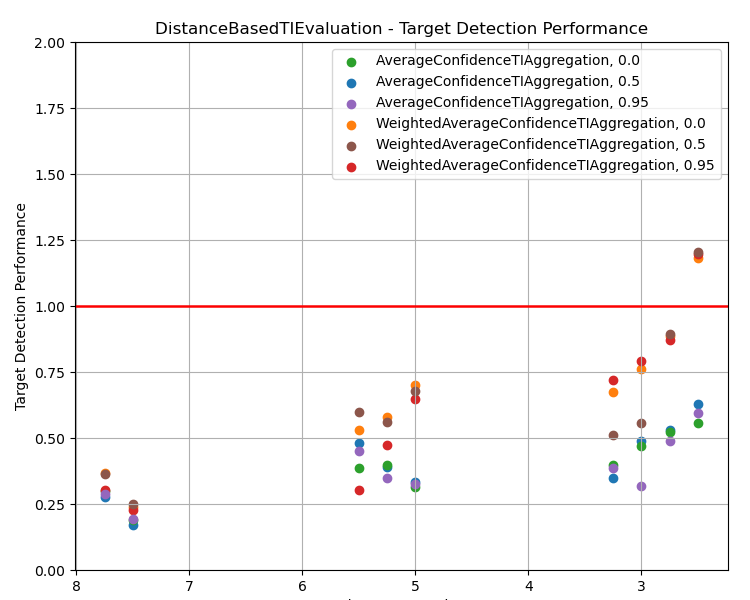
\includegraphics[width=0.7\textwidth]{assets/25_distance_detection_detail.png}
    \caption{$DistanceBasedTIEvaluation$ with 25\% of pre-trusted peers}
    \label{fig:distance-detection-detail-25}
\end{figure}

In Figure~\ref{fig:distance-detection-detail-25} we can clearly see, that there is a situation, even in the hardest environment, where the $DistanceBasedTIEvaluation$ in combination with $AverageConfidenceTIAggregation$ does not have any $tdp$ above the \textit{red line} which means that $tdp < 1$ and that Fides was always able to identify targets correctly even in the worst possible environment.

We included the graph of this case similar to the Figure~\ref{fig:single-simulation-example} with this particular \textit{"winning"} setup in the most hostile environment to the appendix in Figure~\ref{fig:worst-best-scenario}. For the explanation of the graph see Section~\ref{sec:general-overview-of-simulation-output}.

Interestingly, in this particular case, the initial reputation does not affect the final outcome of the simulation, but it does affect the progress as when using an initial reputation higher than $0$, Fides provides wrong scores in the situation when the malicious peers started to lie.
However, it discovers that the peers are lying, which decreases their service trust and is able to eventually recover the correct labels for the targets.
The score value over time for this situation can be seen on the Figure~\ref{fig:missclassification-score-only}.
We included the whole graph in the appendix in Figure~\ref{fig:missclassification-recovery}.

\begin{figure}[ht]
    \centering
    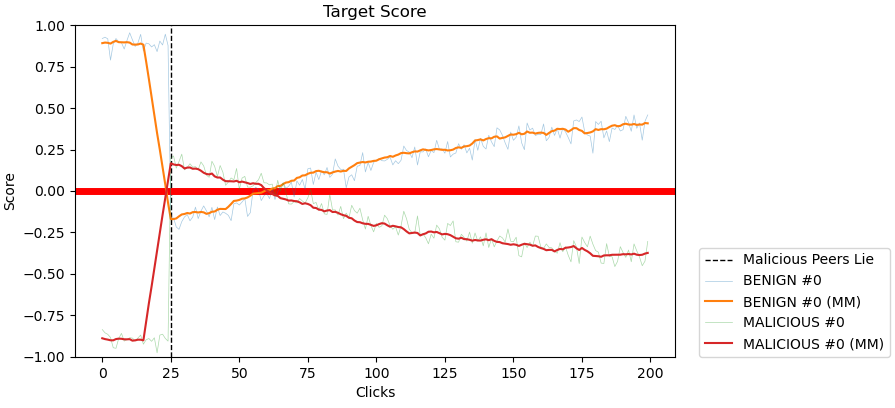
\includegraphics[width=0.9\textwidth]{assets/misclassification_score.png}
    \caption{Score in figure~\ref{fig:missclassification-recovery}.}
    \label{fig:missclassification-score-only}
\end{figure}

It is clear from Figure~\ref{fig:distance-detection-detail-25}, that when Fides used the threat intelligence aggregation method $WeightedAverageConfidenceTIAggregation$~(\ref{subsec:WeightedAverageConfidenceTIAggregation}), it miss-classified the targets in one situation.
Thus, this method does not provide a guarantee that Fides will end up with correct classifications for every target.

The same applies to all other interaction evaluation methods as we can see in the Figure~\ref{fig:performance-all-setups-25-pretrusted} that in the hardest environment, they all classified the targets poorly with all threat intelligence aggregation methods.

\subsection{Resilience Under Different Conditions}
\label{subsec:resilience-under-different-conditions}

We include a similar graph to Figure~\ref{fig:performance-all-setups-25-pretrusted} for the situations with no pre-trusted peers in the appendix in the Figure~\ref{fig:performance-all-setups-0-pretrusted} and then situations with 50\% of pre-trusted peers in the Figure~\ref{fig:performance-all-setups-50-pretrusted}.

With no pre-trusted peers in the network, the results of each configuration vary and they highly depend on the network topology as well as on the knowledge of the local Slips instance.

However, in the case of 50\% pre-trusted peers, one can see that no matter the configuration, Fides was eventually able to determine the correct target classification with a high precision of $tdp \leq 0.7$. Moreover, Fides was able to correctly identify the peer's behavior with the precision of $pbdp \leq 0.2$.

\newpage
\section{Other Findings}
\label{sec:other-findings}

Even though the results from the previous Section~\ref{sec:fides-resilience} suggest that a combination of $DistanceBasedTIEvaluation$ for evaluating the interactions in combination with $AverageConfidenceTIAggregation$ is the best, this is not always true.

For example, recall Figure~\ref{fig:single-simulation-example} from the Section~\ref{sec:general-overview-of-simulation-output}, where the presented situation uses $MaxConfidenceTIEvaluation$ and it is able to correctly detect all types of peers as well as correctly determine the score for the target.
However, if we take the same environment and the only difference is using $DistanceBasedTIEvaluation$ for evaluating interactions, we get the following graph for the service trust in the Figure~\ref{fig:zero-gained-trust}.

\begin{figure}[h]
    \centering
    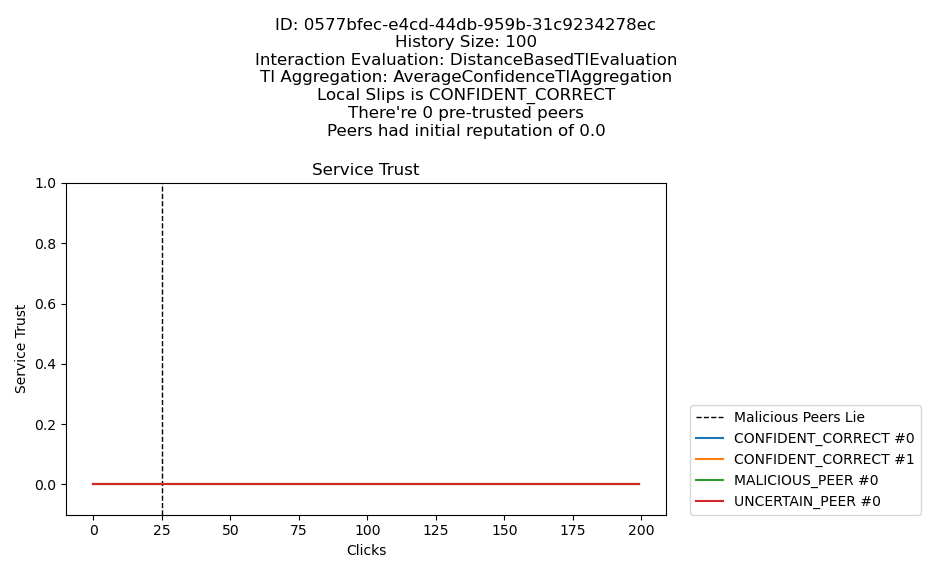
\includegraphics[width=0.8\textwidth]{assets/zero_gained_trust.png}
    \caption{$DistanceBasedTIEvaluation$ in the situation from the figure~\ref{fig:single-simulation-example}}
    \label{fig:zero-gained-trust}
\end{figure}

The graph for confidence as well as target score for the situation from Figure~\ref{fig:zero-gained-trust} can be seen in the appendix in the Figure~\ref{fig:zero-gained-trust-all}.

The service trust graph in Figure~\ref{fig:zero-gained-trust} suggests that Fides didn't gain any trust for any peer in the network.
This happens because the evaluation strategy didn't have enough information at the beginning to evaluate the received data properly.
That leads to peers never gaining any trust and thus not producing any valid outputs because, with no trust, the target score and confidence ended up being $0$ as well.